\chapter{Phase 5 \& 6: Multi-Threading, Dwell Stabilizer and AI Linguistic Bridge}
\label{Chapter 5}

\section{Five-Thread Asynchronous Decoupled Engine Architecture}
To ensure that compute-heavy tasks (neural voice synthesis, translation, grammar polishing, and audio transcription) never cause the 30 FPS camera feed to drop frames, \textbf{SignSpeak Universal} runs across \textbf{five isolated parallel threads} (diagrammed in Figure~\ref{fig:concurrency_threads}):

\begin{figure}[htbp]
    \centering
    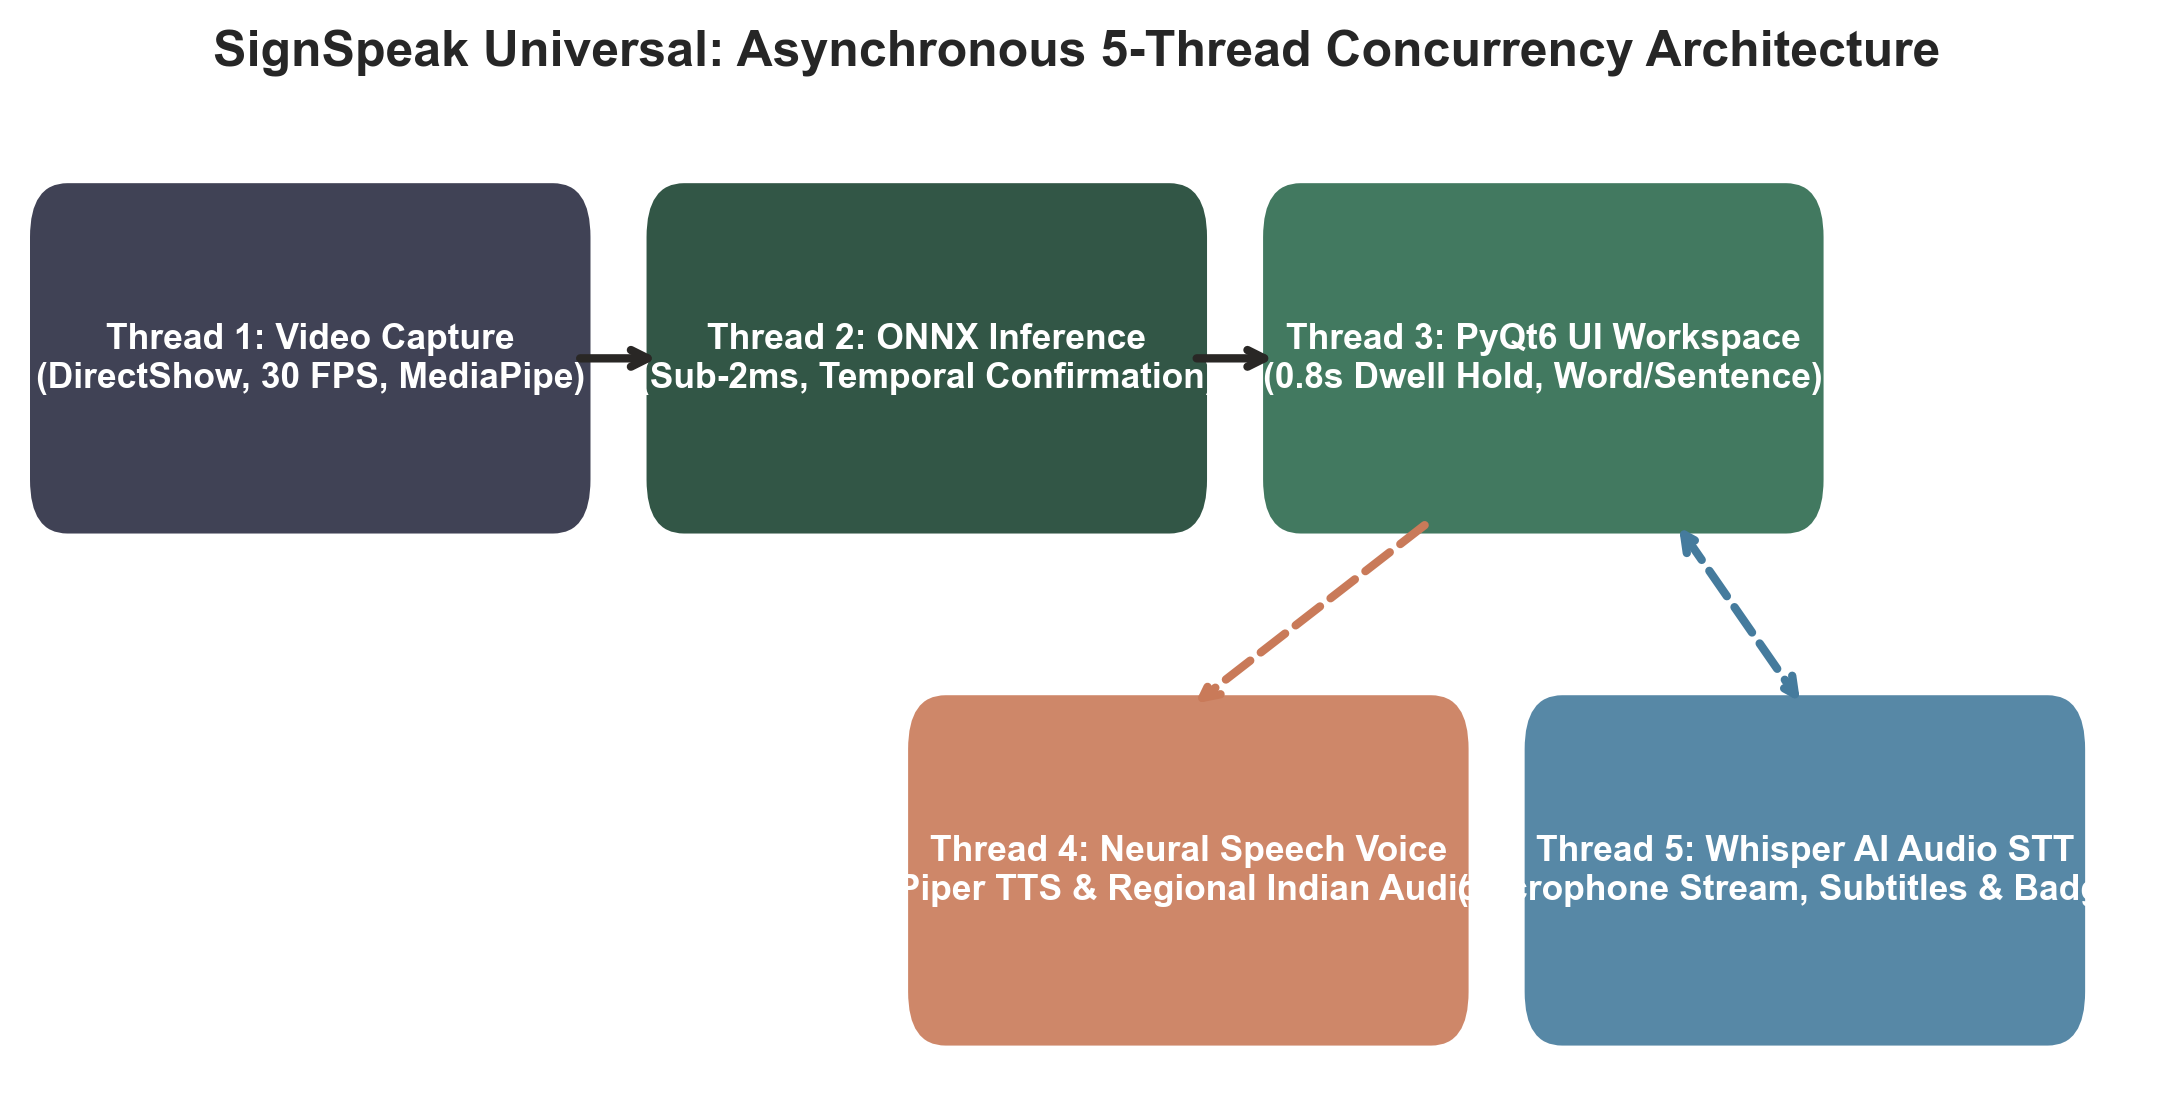
\includegraphics[width=0.92\textwidth]{figures/fig_05_concurrency_threads.png}
    \caption{SignSpeak Universal 5-Thread Asynchronous Concurrency Architecture: Decoupling video capture, sub-2ms ONNX inference, PyQt6 workspace UI, local Piper TTS, and Whisper STT.}
    \label{fig:concurrency_threads}
\end{figure}

\begin{enumerate}
    \item \textbf{\texttt{CaptureThread}:} DirectShow camera capture at 30 FPS, MediaPipe 3D landmark tracking, and 126-dimensional coordinate vector extraction.
    \item \textbf{\texttt{InferenceThread}:} Sub-2ms ONNX letter inference on incoming vectors, with a 4-frame consecutive temporal confirmation filter to prevent visual flickering during hand transitions.
    \item \textbf{\texttt{SignSpeakApp} (Main UI Thread):} Manages the Qt6 desktop workspace, 0.8s dwell hold progress calculation, autocomplete chip rendering, and keyboard event dispatching.
    \item \textbf{\texttt{TTSThread}:} Manages non-blocking local Piper neural voice synthesis (\texttt{en\_US-lessac-medium.onnx}, $<12\text{ ms}$) and regional acoustic voice playback via Windows MCI APIs.
    \item \textbf{\texttt{SpeechToTextThread}:} Streams background microphone audio at 16kHz mono via \texttt{sounddevice}, packaging PCM audio frames for Whisper AI transcription.
\end{enumerate}

\begin{figure}[htbp]
    \centering
    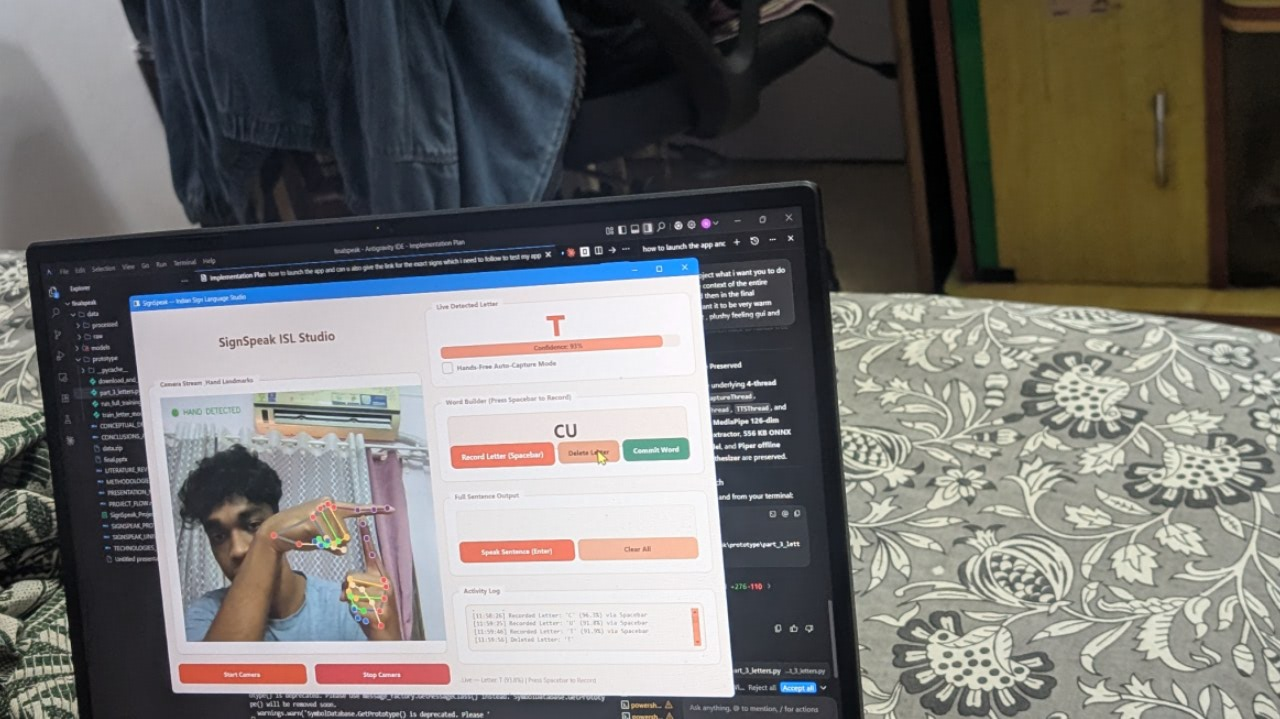
\includegraphics[width=0.88\textwidth]{figures/gallery_photo_1.png}
    \caption{Live Experimental Snapshot: Real-time execution of the SignSpeak desktop application. The student signs the ISL letter `T' (recognized at 93\% confidence), while the active Word Builder constructs the word `CU' with zero camera frame drops.}
    \label{fig:live_desktop_app}
\end{figure}

\section{The 0.8s Steady-Hold Dwell Stabilizer with Hysteresis Lock}
A major ergonomic flaw in conventional sign recognition tools is the requirement for manual mouse clicks or continuous spacebar tapping to capture each letter. This causes severe physical fatigue.

We engineered a \textbf{Hands-Free Steady-Hold Dwell Stabilizer} (modeled as a Finite State Machine in Figure~\ref{fig:dwell_fsm}):
\begin{itemize}
    \item \textbf{0.80s Hold Threshold:} When a user holds a recognizable sign steady with $\ge 50\%$ confidence, an on-screen green progress bar fills smoothly over \textbf{0.80 seconds}.
    \item \textbf{Audio Feedback Confirmation:} When the dwell reaches 100\%, the letter is automatically committed into the active word builder, accompanied by a soft 35ms audio tick (1250 Hz).
    \item \textbf{Anti-Duplication Hysteresis Lock:} Following capture, an internal state lock prevents the letter from repeating until the user either changes their handshape or lowers their hand, completely eliminating unintentional letter stutter.
\end{itemize}

\begin{figure}[htbp]
    \centering
    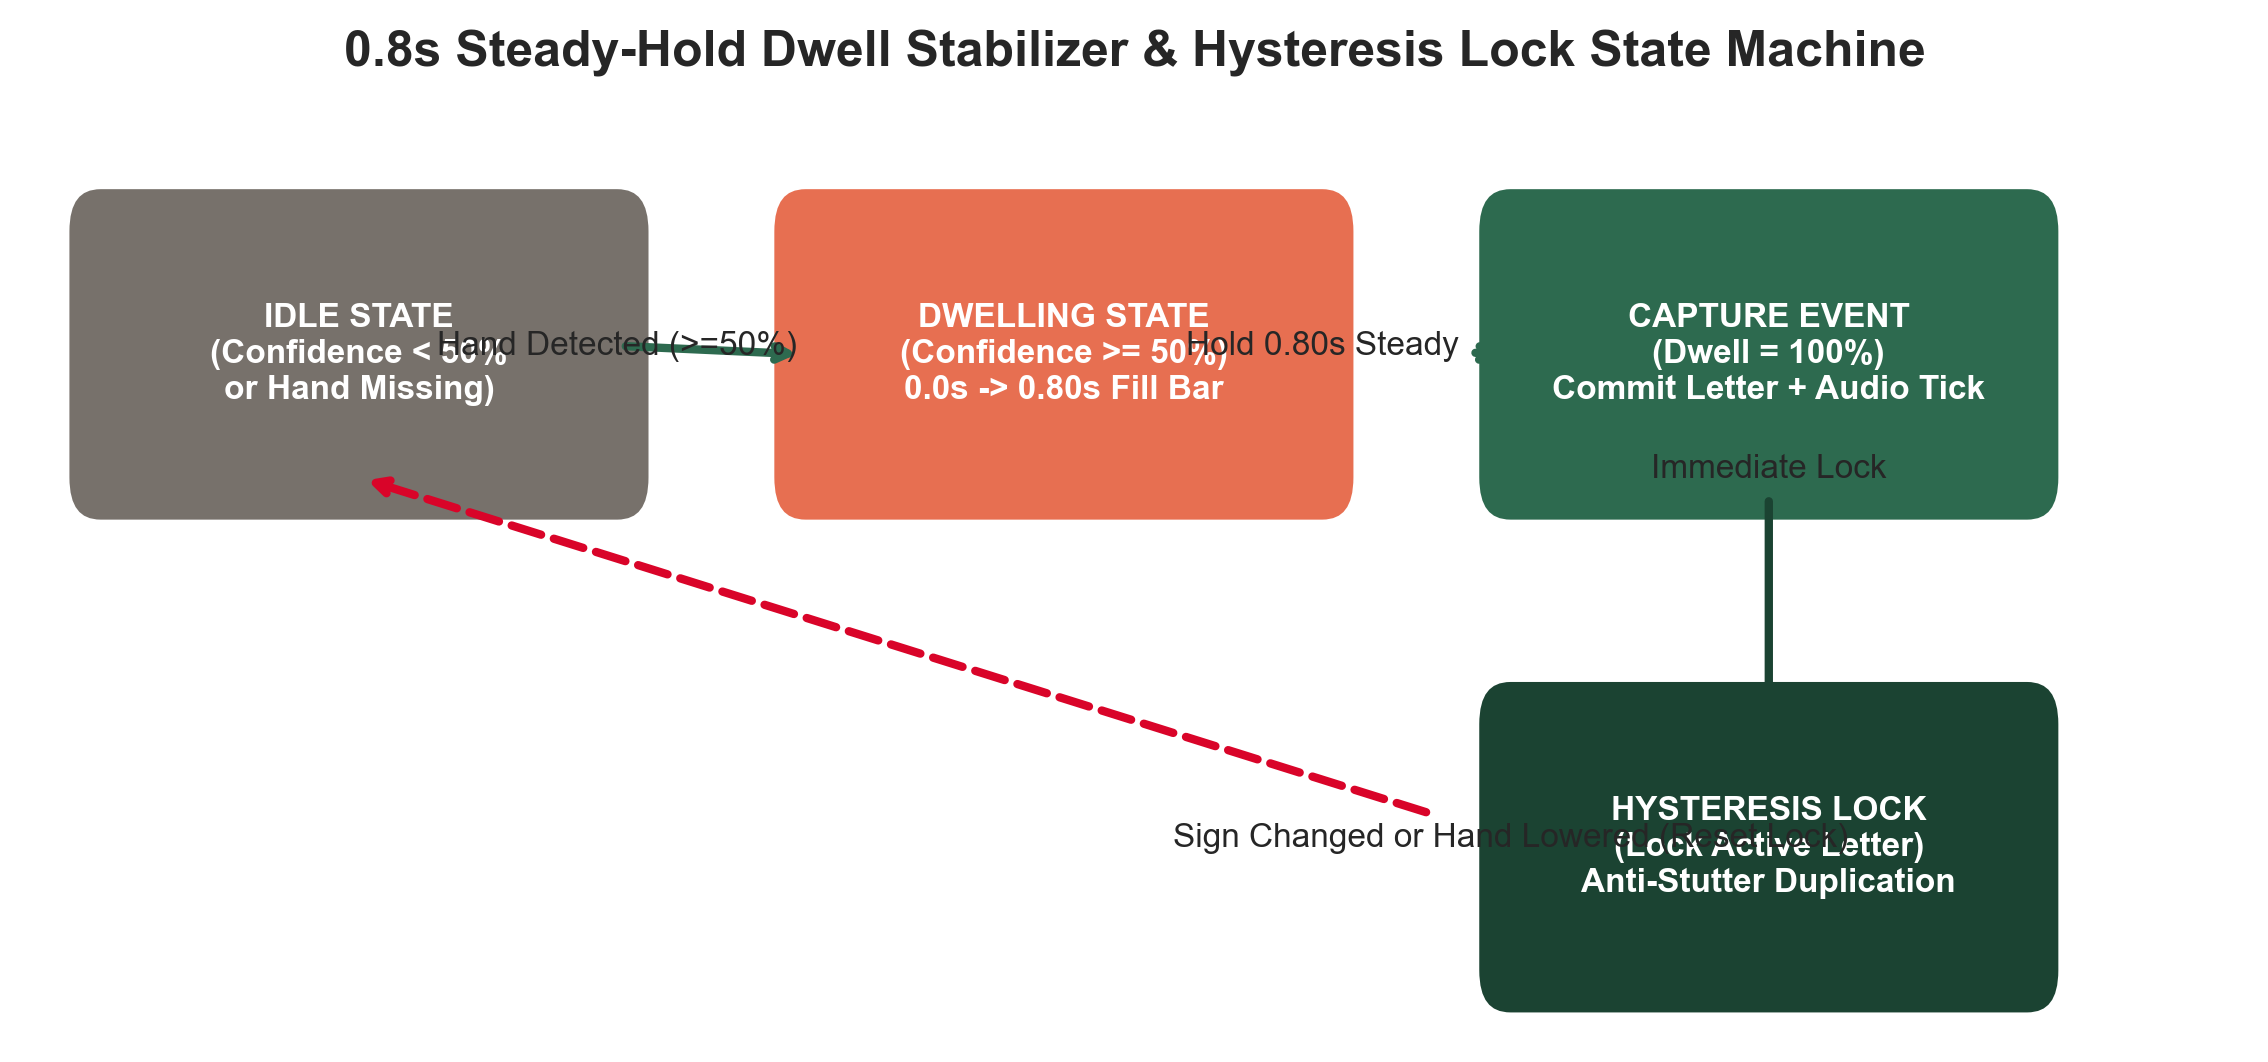
\includegraphics[width=0.88\textwidth]{figures/fig_09_dwell_fsm_diagram.png}
    \caption{Finite State Machine (FSM) diagram of the 0.8s Steady-Hold Dwell Stabilizer showing transition from IDLE to DWELLING, CAPTURE EVENT, and the anti-duplication HYSTERESIS LOCK.}
    \label{fig:dwell_fsm}
\end{figure}

\section{One-Euro Signal Filtering}
To eliminate high-frequency coordinate jitter caused by webcam sensor noise, we implemented an adaptive \textbf{One-Euro Filter} on all 21 keypoints:
\begin{equation}
\alpha = \frac{1}{1 + \frac{\tau}{\Delta t}}, \quad \tau = \frac{1}{2\pi f_c}, \quad f_c = f_{c, \min} + \beta |\dot{x}|
\end{equation}
During slow, stationary gestures, the cutoff frequency $f_c$ drops to $1.0\text{ Hz}$, eliminating jitter completely. During rapid hand transitions, $f_c$ scales up dynamically, ensuring zero perceptible lag.

\section{Ergonomic Keyboard Mechanics}
\begin{itemize}
    \item \textbf{Spacebar Word Commit:} Commits the formed word into the spoken sentence line and resets the word builder.
    \item \textbf{Smart Backspace:} Deletes the last character; if the active word builder is empty, it intelligently pulls the previous word back from the sentence line for editing.
    \item \textbf{Escape Buffer Reset:} Instantly clears both word and sentence buffers.
\end{itemize}

\section{Gboard-Style AI Autocomplete Strip}
To accelerate communication, we built a \textbf{Gboard-Style AI Autocomplete Strip} displaying three clickable suggestion chips (e.g., \texttt{[ 1  HELLO ]}, \texttt{[ 2  HELP ]}, \texttt{[ 3  HEAR ]}).
\begin{itemize}
    \item \textbf{Dual-Tier Prediction:} Integrates an instant ($<0.1\text{ ms}$) local offline frequency dictionary with an asynchronous background Groq Cloud LLM worker that predicts words based on active prefix and sentence context.
    \item \textbf{One-Touch Hotkeys (\texttt{1}, \texttt{2}, \texttt{3}):} Pressing standard number keys or numeric keypad keys instantly autocompletes and commits the word.
\end{itemize}

\section{1-Click AI Sign Grammar Polish and Non-Destructive Revert}
To bridge the gap between telegraphic sign glosses (e.g., \textit{``ME WATER DRINK WANT''}) and natural conversational speech:
\begin{itemize}
    \item Pressing \textbf{\texttt{Ctrl + P}} (or clicking \texttt{Polish}) automatically commits any active word and sends the full sentence to our background AI worker, converting the gloss into a fluent sentence (\textit{``I want to drink water.''}) in $\sim 150\text{ ms}$.
    \item \textbf{\texttt{Ctrl + Z} Revert:} Non-destructively restores the exact original raw signed glosses at any time.
    \item \textbf{Auto-Polish on Speak:} Automatically converts sign syntax right before voice synthesis when enabled.
\end{itemize}

\begin{figure}[htbp]
    \centering
    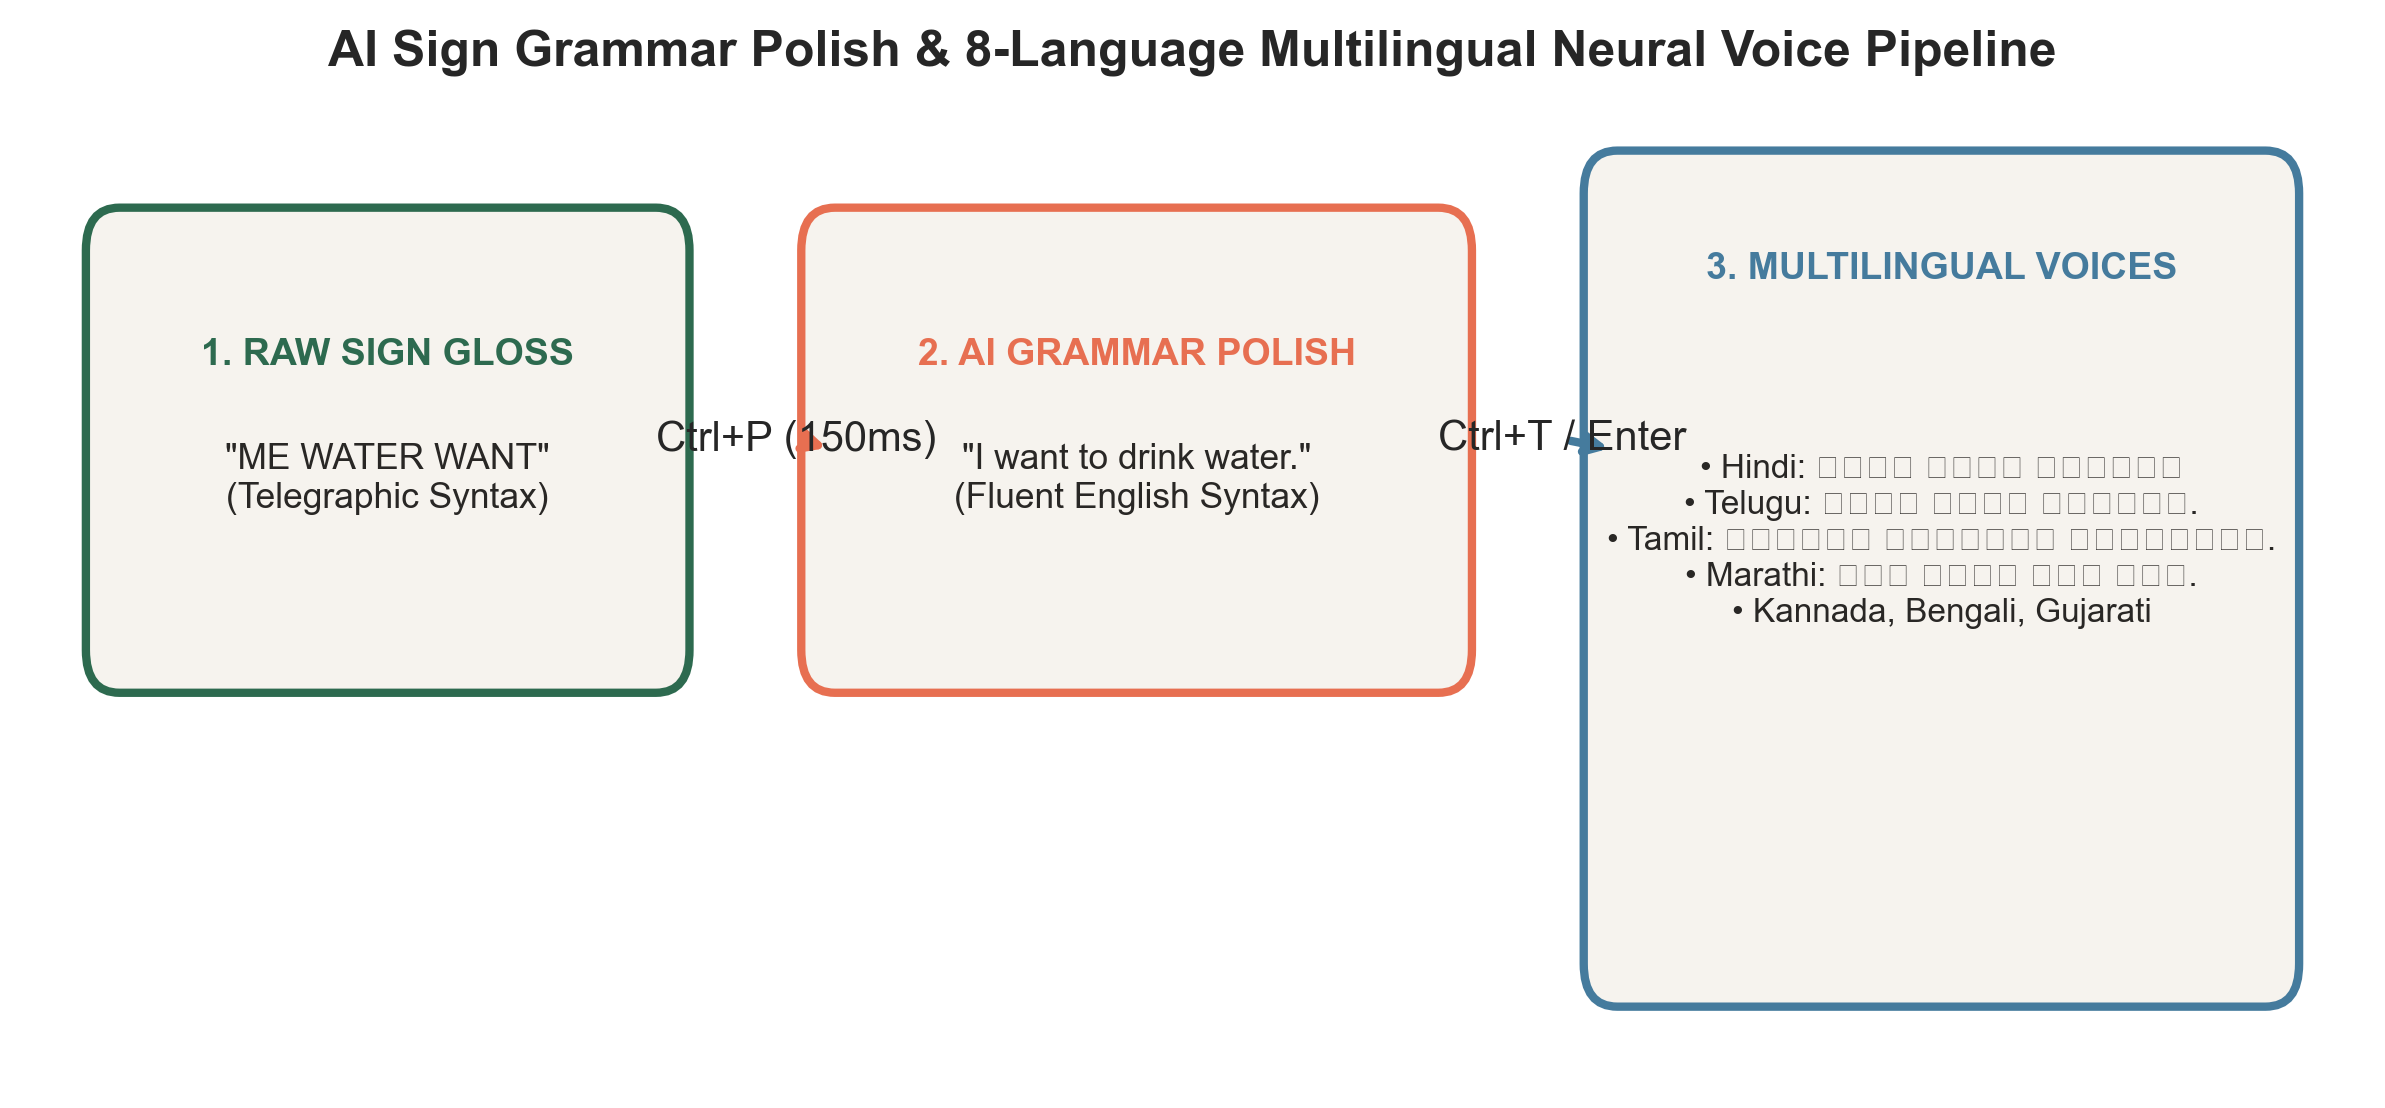
\includegraphics[width=0.92\textwidth]{figures/fig_10_multilingual_voice_pipeline.png}
    \caption{SignSpeak AI Linguistic Pipeline: Transforming raw telegraphic sign glosses into fluent English sentences via 1-Click Polish (\texttt{Ctrl+P}) and synthesizing 8 Indian regional neural speech voices (\texttt{Ctrl+T} / \texttt{Enter}).}
    \label{fig:multilingual_pipeline}
\end{figure}

\section{Multilingual Indian Regional Speech Engine (8 Languages)}
To empower signers across India, we built a multilingual regional speech engine (diagrammed in Figure~\ref{fig:multilingual_pipeline}) supporting \textbf{8 languages}: English, Hindi, Telugu, Tamil, Marathi, Kannada, Bengali, and Gujarati.
\begin{itemize}
    \item \textbf{1-Click Translate (\texttt{Ctrl + T}):} Translates the signed sentence into the selected Indian script with instant visual and audio feedback.
    \item \textbf{Dynamic Regional Speak (\texttt{Enter}):} The Speak button dynamically updates (e.g., \texttt{[ 🔊 Speak in Hindi  Enter ]}) and automatically translates and vocalizes in the target native voice with one click.
\end{itemize}
